\subsection{Ετερογενής Αρχιτεκτονική}
\subparagraph{}
Η ετερογενής αρχιτεκτονική είναι ένα σύνολο προδιαγραφών που επιτρέπουν την ενσωμάτωση κεντρικών μονάδων επεξεργασίας  \emph{\en{(CPU)}} και μονάδων επεξεργασίας γραφικών στον ίδιο δίαυλο, με κοινόχρηστη μνήμη και διεργασίες\cite{toms_hardware}.

Οι μονάδες επεξεργασίας γραφικών βελτιώνουν σημαντικά την απόδοση των προγραμμάτων, με αποτέλεσμα τον πολλαπλασιάσμό της ζήτησης τους. Η αύξηση της δημοτικότητας των ετερογενών αρχιτεκτονικών σε όλους τους τύπους υπολογιστών είχε αξιοσημείωτο αντίκτυπο στην ανάπτυξη λογισμικών υψηλών προδιαγραφών.

Για την εκμετάλλευση των ετερογενών συστημάτων, οι χρήστες πρέπει να κατασκευάζουν λογισμικό που εκτελεί τμήματα κώδικα σε διαφορετικές συσκευές. Τέτοια τμήματα αποτελούν οι βρόγχοι επανάληψης, που χρησιμοποιούνται ευρέως για την δημιουργία λογισμικών.

Ωστόσο, τα μοντέλα προγραμματισμού για ετερογενή συστήματα είναι δύσκολο να χρησιμοποιηθούν λόγω της αυξημένης δυσκολίας διαχείρισής τους. Συνήθως, τμήματα κώδικα γράφονται σε δύο εκδόσεις, μία φορά για τον επεξεργαστή γενικού σκοπού και μια για τον επιταχυντή. Η έκδοση του επιταχυντή γράφεται γλώσσα χαμηλότερου επιπέδου. Η συντήρηση και ανάπτυξη διπλού κώδικα, αποτελεί ένα από τα μεγαλύτερα προβλήματα στην έννοια του προγραμματισμού.

Για τις ανάγκες διευκόλυνσης, το \emph{\en{OpenMP}} επέκτεινε τις λειτουργίες του με σκοπό την υποστήριξη και ευρεία χρήση τέτοιων τύπων συστημάτων\cite{barbara}. Τα αποτελέσματα της εργασίας αρχικά δημοσιεύτηκαν στην έκδοση 4.0 και εξελίχθηκαν περαιτέρω στην έκδοση 4.5. Οι χρήστες μπορούν πλέον να χρησιμοποιήσουν τη διεπαφή για τη δημιουργία λογισμικών γραμμένων με γλώσσες προγραμματισμού υψηλότερου επιπέδου και εκτελέσιμων από συσκευές επεξεργασίας γραφικών. Ετσι επιτυγχάνεται η διατήρηση μίας μόνο έκδοσης του κώδικα, η οποία μπορεί να τρέξει είτε σε μονάδα επεξεργασίας γραφικών ή σε επεξεργαστή γενικής χρήσης\emph{\en{CPU}}.

Με τον όρο συσκευή στόχου, εννοείται ένας υπολογιστικός πόρος, στον οποίο μπορεί να εκτελεστεί μια περιοχή κώδικα. Παραδείγματα τέτοιων συσκευών είναι \emph{\en{GPU, CPU, DSP, FPGA}} κ.α. Οι συσκευές στόχου έχουν τα δικά τους νήματα, των οποίων η μετεγκατάσταση σε άλλες συσκευές δεν είναι δυνατή. Η εκτέλεση του προγράμματος ξεκινάει από την κεντρική συσκευή (\emph{\en{host device}}. Η κεντρική συσκευή είναι υπεύθυνη για την μεταφορά του κώδικα και των δεδομένων στον επιταχυντή (συσκευή στόχου).

\selectlanguage{english}
\begin{lstlisting}[language=C++, caption={\el{Παράδειγμα εκτέλεσης κώδικα στη συσκευή στόχου}} , frame=tlrb]{Name}
 void add_arrays(double *A, double *B, double *C, size_t size) {
     size_t i = 0;
 #pragma omp target map(A, B, C)
     for (i = 0; i < size; ++i) {
             C[i] = A[i] + B[i];
     }
 }
\end{lstlisting}
\selectlanguage{greek}
\clearpage
Οπως δείχνει το παραπάνω παράδειγμα, ένα νήμα του εξυπηρετητή (κύρια συσκευή - \emph{\en{host}}) συναντάει την οδηγία \emph{\en{\textbf{target}}}. To τμήμα κώδικα που ακολουθεί μεταφέρεται και εκτελείται στη συσκευή του επιταχυντή, αν αυτός υπάρχει. Απο προεπιλογή, το νήμα που συναντά την οδηγία περιμένει την ολοκλήρωση της εκτέλεσης της παράλληλης περιοχής, προτού συνεχίσει.

Πριν ένα καινούργιο νήμα που βρίσκεται στη συσκευή στόχου αρχίσει να εκτελεί την περιοχή που περικλείεται στην οδηγία \emph{\en{target}}, οι μεταβλητές  \emph{\en{A, B, C}} \emph{"αντιστοιχίζονται"} στον επιταχυντή. Η φράση \emph{\en{mapped}} είναι το εργαλείο που χρησιμοποιεί το \emph{\en{OpenMP}} για να εξασφαλίσει τον πρόσβαση του της συσκευής στόχου, στις μεταβλητές αυτές.


\subsubsection{Το αρχικό νήμα της συσκευής προορισμού}
\subparagraph{}
Το νήμα που ξεκινάει την εκτέλεση ενός προγράμματος, ονομάζεται κύριο νήμα και ανήκει πάντα στην κεντρική συσκευή. Με άλλα λόγια, ένα πρόγραμμα σε μια αρχιτεκτονική ετερογενούς προγραμματισμού, δε ξεκινάει ποτέ από τη συσκευή στόχου.

Με την εισαγωγή της οδηγίας \emph{\en{target}} στο \emph{\en{OpenMP}} 4.0, πολλαπλά αρχικά νήματα μπορούν να δημιουργηθούν κατά τη διάρκεια εκτέλεσης ενός προγράμματος. Την εκτέλεση του τμήματος κώδικα στη συσκευή προορισμού, την αναλαμβάνει ένα νέο αρχικό νήμα και όχι το νήμα που συνάντησε την οδηγία \emph{\en{target}}. Το νήμα αυτό μπορεί να συναντήσει οδηγίες παραλληλισμού και να δημιουργήσει υποομάδες νημάτων.
\ \\
\begin{figure}[h]
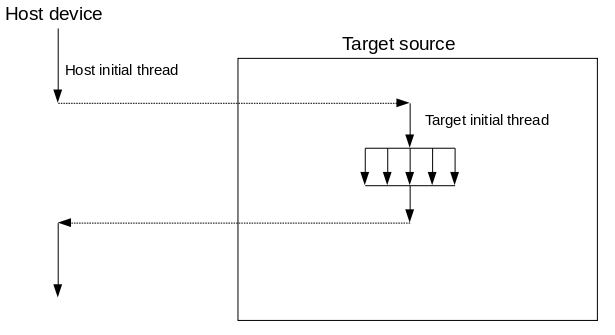
\includegraphics[width=\textwidth]{heter_1}
\centering
\captionsetup{justification=centering, singlelinecheck=false}
	\caption{Διάγραμμα ομάδων νημάτων σε ετερογενή αρχιτεκτονική}
\label{fig:heter_1}
\end{figure}
\clearpage




\subsubsection{Μοντέλο μνήμης ετερογενούς αρχιτεκτονικής}
\subparagraph{}
Στις επόμενες παραγράφους, ακολουθεί μια περιγραφή του μοντέλου μνήμης της ετερογενούς αρχιτεκτονικής, περιγράφονται έννοιες που σχετίζονται με τις μεταβλητές και η γνώση του θεωρητικού υπόβαθρου καθίσταται απαραίτητη για την ορθή υλοποίηση προγραμμάτων σε τέτοιες αρχιτεκτονικές.

\paragraph{Η οδηγία \emph{\en{map}}}
\subparagraph{}
Οπως τα νήματα των εξυπηρετητών, έτσι και τα νήματα που δημιουργούνται στις συσκευές στόχου μπορούν να έχουν ιδιωτικές μεταβλητές. Αντίγραφα μεταβλητών στη συσκευή στόχου με χαρακτηριστικό ιδιωτικής μνήμης, δημιουργούνται όταν η οδηγία \emph{\en{target}} ακολουθείται από τη φράση \emph{\en{private} ή \en{firstprivate}}.

Στις αρχιτεκτονικές ετερογενούς προγραμματισμού και σε επίπεδο υλικού, ο εξυπηρετητής με τον επιταχυντή μπορεί να μοιράζονται κοινόχρηστη φυσική μνήμη.
Η φράση \emph{\en{map}} χρησιμοποιείται για την αντιστοίχιση δεδομένων ανάμεσα στις δύο συσκευές, αποκρύπτοντας παράλληλα χαρακτηριστικά της φυσικής υλοποίησης. Για παράδειγμα, όταν οι δυο συσκευές δεν έχουν κοινόχρηστη φυσική μνήμη, η μεταβλητή αντιγράφεται στον επιταχυντή. Αντίθετα, στην περίπτωηση της υλοποίησης με κοινόχρηστη μνήμη, δεν απαιτείται δημιουργία αντίγραφου.  Η φράση \emph{\en{map}} απαλλάσει τον χρήστη από τον έλεγχο των χαρακτηριστικών της υλοποίησης σε επίπεδο υλικού, και η διεπαφή ενεργεί ανάλογα με την αρχιτεκτονική που χρησιμοποιείται.
\\

\begin{table}[htbp]
\captionsetup{justification=raggedright,
singlelinecheck=false
}
\caption{Ενέργειες που εκτελούνται από την οδηγία\en{\emph{map}} ανάλογα με το είδος της αρχιτεκτονικής μνήμης}
\def\arraystretch{1.5}
\begin{tabular}{| p{0.25\textwidth} | p{0.25\textwidth}|  p{0.25\textwidth} |  p{0.25\textwidth}|}
\hline
\cellcolor[HTML]{D0D0D0} & \textbf{\en{memory allocation}} \cellcolor[HTML]{D0D0D0} & \textbf{\en{copy}}\cellcolor[HTML]{D0D0D0} & \textbf{\en{flush}} \cellcolor[HTML]{D0D0D0} \\
\hline
\textbf{Διαμοιρασμένη Μνήμη} & Ναι & Ναι & Ναι \\
\hline
\textbf{Κοινόχρηστη Mνήμη} & Οχι & Οχι & Ναι \\
\hline
\end{tabular}
\end{table}

\paragraph{Περιβάλλον δεδομένων συσκευής}
\subparagraph{}
Κάθε επιταχυντής έχει ένα περιβάλλον μνήμης στο οποίο περιέχεται το σύνολο των μεταβλητών που είναι προσβάσιμες από νήματα που ενεργούν σε αυτή τη συσκευή. Η οδηγία \emph{\en{(map)}} διασφαλίζει ότι η μεταβλητή μεταφέρεται απο τον εξυπηρετητή, στο περιβάλλον δεδομένων του επιταχυντή και είναι προσβάσιμη από αυτόν.

Ανάλογα με την αρχιτεκτονική και τη διαθεσιμότητα κοινόχρηστης μνήμης μεταξύ του εξυπηρετητή \emph{\en{(host)}} και της συσκευής προορισμού, η πρωτότυπη μεταβλητή που δημιουργήθηκε στον εξυπηρετητή και η αντίστοιχη της συσκευής προορισμού είναι είτε η ίδια μεταβλητή που βρίσκεται στη κοινόχρηστη μνήμη των δυο συσκευών ή αντίγραφα σε διαφορετικές θέσεις μνήμης. Στη δεύτερη περίπτωση, απαιτούνται εργασίες αντιγραφής και ενημέρωσης για να διατηρηθεί η συνέπεια μεταξύ των δυο θέσεων.

Η βελτιστοποίηση της ποσότητας της μεταφοράς δεδομένων ανάμεσα στις δυο συσκευές, αποτελεί κρίσιμο σημείο για την επίτευξη καλύτερης απόδοσης στις ετερογενείς αρχιτεκτονικές.
Η συνεχείς αντιστοίχιση μεταβλητών που επαναχρησιμοποιούνται είναι αναποτελεσματική και οδηγεί σε πτώση της απόδοσης.

\paragraph{Δείκτες μεταβλητών συσκευής}
\subparagraph{}
Αν ο εξυπηρετητής και ο επιταχυντής δεν μοιράζονται την κοινόχρηστη μνήμη, οι τοπικές μεταβλητές τους βρίσκονται σε διαφορετικές θέσεις μνήμης. Όταν μια μεταβλητή αντιστοιχίζεται στο περιβάλλον δεδομένων ενός επιταχυντή, γίνεται μια αντιγραφή και η καινούργια μεταβλήτή ειναι διαφορετική από την μεταβλητή του εξυπηρετητή.

Οι διευθύνσεις μνήμης αποθηκεύονται σε μεταβλητές που ονομάζονται δείκτες (\emph{\en{pointers}}. Ένα νήμα του εξυπηρετητή δε μπορεί να έχει πρόσβαση σε μνήμη μέσω ενός δείκτη που περιέχει διεύθυνση μνήμης του επιταχυντή. Ακόμη, ο επιταχυντής και ο εξυπηρετητής μπορεί να έχουν διαφορετική αρχιτεκτονική, δηλαδή ένας τύπος μεταβλητής μπορεί να είναι διαφορετικού μεγέθους ανάμεσα στις δύο συσκευές.

Ο δείκτης συσκευής \emph{\en{(device pointer)}} είναι ένας δείκτης που αποθηκεύεται στον εξυπηρετητή και περιέχει την διεύθυνση μνήμης στο περιβάλλον δεδομένων του επιταχυντή. Το \emph{\en{OpenMP}} παρέχει ρουτίνες και οδηγίες που καθιστούν εφικτή τη δέσμευση μνήμης στο περιβάλλον του επιταχυντή μέσω του εξυπηρετητή, όπως φαίνεται στο παρακάτω παράδειγμα:


\selectlanguage{english}
\begin{lstlisting}[language=C++, caption={\el{Παράδειγμα} taskwait} , frame=tlrb]{Name}
int device = omp_get_default_device();
char *device_ptr = omp_target_alloc(n, device);
#pragma omp target is_device_ptr (device_ptr)
for (int j=0; j<n ; j++)
	*device_ptr++ = 0;
\end{lstlisting}
\selectlanguage{greek}
\clearpage


\subsubsection{Η οδηγία \en{target}}
\subparagraph{}
Σκοπός της οδηγίας \emph{\en{target}} είναι η μεταφορά και εκτέλεση ενός τμήματος κώδικα στον επιταχυντή. Η εκτέλεση γίνεται από ένα αρχικό νήμα στη συσκευή. Σε περίπτωση έλλειψης επιταχυντή στο σύστημα, ο κώδικας που προορίζεται να εκτελεστεί εκεί μέσω της οδηγίας \emph{\en{target}} θα εκτελεστεί στον εξυπηρετητή αγνοώντας τις οδηγίες \emph{\en{\#pragma}}.

\selectlanguage{english}
\begin{lstlisting}[language=C++, caption={\el{Σύνταξη οδηγίας} target} , frame=tlrb]{Name}
#pragma omp target [clause[[,] clause]...]
\end{lstlisting}
\selectlanguage{greek}

\selectlanguage{english}
\begin{lstlisting}[language=C++, caption={\el{Παράδειγμα εκτέλεσης στον επιταχυντή} } , frame=tlrb]{Name}
void test() {
	int flag = 0;
	#pragma omp target map(flag)
	{
		flag = !omp_is_initial_device() ? 1 : 2;
	}
	if (flag == 1) {
		printf("Running on accelerator\n");
	} else if (flag == 2) {
		printf("Running on host\n");
	}
}
\end{lstlisting}
\selectlanguage{greek}
\ \\
Η οδηγία \emph{\en{target}} δημιουργεί μια διεργασία που εκτελείται στον επιταχυντή. Η διεργασία για τον εξυπηρετητή ολοκληρώνεται όταν ολοκληρωθεί η εκτέλεση στον επιταχυντή. Οι φράσεις \emph{\en{nowait}} και \emph{\en{depend}} επηρεάζουν τον τύπο και την ασύγχρονη συμπεριφορά της διεργασίας. Από προεπιλογή, η διεργασία στόχου περιλαμβάνει φράγμα εκτέλεσης στο τέλος της. Το νήμα που τη συναντά περιμένει μέχρι την ολοκλήρωση της εκτέλεσής της.

Οι δείκτες μεταβλητών που εισάγονται στη φράση \emph{\en{map}}, είναι ιδιωτικές (\emph{\en{private}}) μέσα στη συσκευή στόχου. Οι ιδιωτικές μεταβλητές δείκτη διεύθυνσης αρχικοποιούνται με την τιμή της διεύθυνσης του επιταχυντή.

Οι φράσεις που υποστηρίζονται από την οδηγία είναι:

\selectlanguage{english}
\begin{lstlisting}[language=C++, caption={\el{Φράσεις οδηγίας} \emph{\en{target}} } , frame=tlrb]{Name}
if (/target:] scalar-expression)
map ([[map-type-modifier[, map-type:] list]
device (integer-expression)
private (list)
firstprivate (list)
is_device_ptr (list)
defaultmap( tofrom:scalar)
nowait
depend(dependence-type: list)
\end{lstlisting}
\selectlanguage{greek}

\subsubsection{Η οδηγία \en{target teams}}
\subparagraph{}
Η οδηγία \emph{\en{target teams}} κατασκευάζει ομάδες νημάτων (\emph{\en{league}}) που λειτουργούν σε έναν επιταχυντή. Η κάθε ομάδα αποτελείται από ένα νήμα, το αρχικό. Η λειτουργία αυτή είναι παρόμοια με μια οδηγία \emph{\en{parallel}}. H διαφορά σε αυτή την περίπτωση είναι οτι δημιουργούνται ομάδες που αρχικά απότελούνται απο ένα νήμα και στη συνέχεια τα νήματα της ομάδας πολλαπλασιάζονται. Νήματα διαφορετικών ομάδων δε συγχρονίζονται μεταξύ τους.

Όταν μια παράλληλη περιοχή συναντάται από μια ομάδα, τότε το αρχικό νήμα γίνεται κύριο σε μια νέα υποομάδα. Το αποτέλεσμα είναι ένα σύνολο υποομάδων, οπου κάθε υποομάδα αποτελείται από ένα ή περισσότερο νήματα. Αυτή η δομή χρησιμοποιείται για να εκφράζεται ένας τύπος χαλαρού παραλληλισμού, όπου ομάδες νημάτων εκτελούν παράλληλα, αλλά με μικρή αλληλεπίδραση μεταξύ τους.

\begin{figure}[h]
\includegraphics[width=0.75\textwidth]{targetteams}
\centering
\captionsetup{justification=centering, singlelinecheck=false}
	\caption{\emph{\en{Target teams}}\cite{targettteams}}
\label{fig:targetteams}
\end{figure}


\selectlanguage{english}
\begin{lstlisting}[language=C++, caption={\el{Φράσεις οδηγίας} \emph{\en{target}} } , frame=tlrb]{Name}
num_teams (integer-expression)
threadJimit (integer-expression)
default(shared I none)
private (list)
firstprivate (list)
shared (list)
reduction (reduction-identifier : list)
\end{lstlisting}
\selectlanguage{greek}
\clearpage
\subsubsection{Η οδηγία \en{distribute}}
\subparagraph{}


\selectlanguage{english}
\begin{lstlisting}[language=C++, caption={\el{Σύνταξη οδηγίας} \emph{\en{distribute}} } , frame=tlrb]{Name}
#pragma omp distribute {clause[[,} clause}. . . j
	for-loops
\end{lstlisting}
\selectlanguage{greek}


\selectlanguage{english}
\begin{lstlisting}[language=C++, caption={\el{Φράσεις υποστηριζόμενες από την οδηγία} \emph{\en{distribute}} } , frame=tlrb]{Name}
private {list)
firstprivate {list)
lastprivate {list)
collapse (n)
dist_schedule {kind[, chunk_sizej)
\end{lstlisting}
\selectlanguage{greek}

Η οδηγία \emph{\en{distribute}} χρησιμοποιείται για τον δήλωση διαμοιρασμού των επαναλήψεων ενός βρόγχου στα αρχικά νήματα των ομάδων που δημιουργήθηκαν από την οδηγία \emph{\en{target teams}}. Η οδηγία δεν περιλαμβάνει υπονοούμενο φράγμα εργασιών στο τέλος της, πράγμα που σημαίνει οτι τα κύρια νήματα των ομάδων δε συγχρονίζονται στο τέλος της οδηγίας.

Η φράση \emph{\en{distschedule}} καθορίζει τον τρόπο που διαμοιράζονται οι επαναλήψεις σε τμήματα. Συγκριτικά με την οδηγία \emph{\en{for}}, η \emph{\en{distribute}} έχει πιθανότητες για καλύτερη απόδοση καθώς ο μεταγλωττιστής μπορεί να πετύχει καλύτερο επίπεδο βελτιστοποίησης.



\subsubsection{Σύνθετες οδηγίες επιταχυντών}
\subparagraph{}

Οι συνδυασμένες οδηγίες είναι ισοδύναμες με τις επιμέρους  οδηγίες από τις οποίες αποτελούνται. Για παράδειγμα, η οδηγία \emph{\en{parallel for}} έχει την ιδια σημασία με την \emph{\en{parallel}} ακολουθούμενη από την οδηγία \emph{\en{for}}. Παρόλα αυτά, ορισμένες φορές οι συνδυασμένες οδηγίες μπορούν να επιτύχουν καλύτερες επιδόσεις.
Σε αυτή την παράγραφο, οι οδηγίες χωρίζονται σε δύο κατηγορίες, τις συνδυασμένες με \emph{\en{target}} και αυτές που συνδυάζονται με \emph{\en{target teams}}.

\selectlanguage{english}
\begin{lstlisting}[language=C++, caption={\el{Συνδυασμένες οδηγίες συσκευής στόχου}} , frame=tlrb]{Name}
#pragma omp target parallel [clause[[,] clause]...]
	structured block

#pragma omp target parallel for [clause[[,] clause]...]
	for-loops
	
#pragma omp target parallel for simd [clause[[,] clause]...]
	for-loops
	
#pragma omp target simd [clause[[,] clause]...]
	for-loops
\end{lstlisting}
\selectlanguage{greek}

\clearpage
\selectlanguage{english}
\begin{lstlisting}[language=C++, caption={\el{Συνδυασμένες οδηγίες διαμοιρασμού εργασιών στη συσκευή στόχου}} , frame=tlrb]{Name}
#pragma omp distribute parallel for [clause[[,] clause]...]
	for-loops
#pragma omp distribute simd [clause[[,] clause]...]
	for-loops
#pragma omp distribute parallel for simd [clause[[,] clause]...]
	for-loops
\end{lstlisting}
\selectlanguage{greek}

\subsubsection{Φράσεις οδηγίας \emph{\en{map}}}
\subparagraph{}
\selectlanguage{english}
\begin{lstlisting}[language=C++, caption={\el{Σύνταξη οδηγίας} map} , frame=tlrb]{Name}
map ([[map-type-modifier[,}} map-type:} list)

\end{lstlisting}
\selectlanguage{greek}
\selectlanguage{english}
\begin{lstlisting}[language=C++, caption={\el{Αποδεκτοί τύποι αντιστοίχισης}} , frame=tlrb]{Name}
	alloc
	to
	from
	tofrom -> default
	release
	delete
\end{lstlisting}
\selectlanguage{greek}

Η αντιστοίχιση μεταβλητών στον επιταχυντή, χωρίζεται σε τρεις φάσεις:
\begin{enumerate}
  \item Η φάση \emph{\en{map-enter}} στην αρχή της εκτέλεσης της οδηγίας \emph{\en{target}}, όπου οι μεταβλητή αντιστοιχίζεται στον επιταχυντή. Σε αυτή, δεσμεύεται μνήμη του επιταχυντή για την αποθήκευση της μεταβλητής και αντιγράφεται από τον εξυπηρετητή.
  \item Η φάση υπολογισμού, που προκύπτει όταν κατά τη διάρκεια εκτέλεσης της παράλληλης περιοχής, τα νήματα που εκτελούν το πρόγραμμα αποκτούν πρόσβαση στην αντιστοιχισμένη μεταβλητή.
  \item Η φάση εξόδου όπου ολοκληρώνεται η αντιστοίχιση των μεταβλητών στον επιταχυντή. Η τιμή της μεταβλητής στον επιταχυντή αντιγράφεται στην αντίστοιχη θέση του εξυπηρετητή. Η δεσμευμένη μνήμη του επιταχυντή ελευθερώνεται.
\end{enumerate}

Οι φάσεις \textbf{1} και \textbf{3} διαχειρίζονται την αποθήκευση και την αντιγραφή των μεταβλητών ανάμεσα σε δυο συσκευές. Ο τύπος της αντιστοίχισης επηρεάζει την αντιγραφή μεταβλητών στον επιταχυντή ή τον εξυπηρετητή. Ο καθορισμός του τύπου αντιστοίχισης επηρεάζει την απόδοση του κώδικα.
\clearpage

\begin{table}[htbp]
\captionsetup{justification=raggedright,
singlelinecheck=false
}
\caption{Απαιτούμενη αντιγραφή για κάθε τύπο μεταβλητής κατά τις φάσεις εισόδου-εξόδου}
\def\arraystretch{1.5}
\begin{tabular}{| p{0.25\textwidth} | p{0.25\textwidth}|  p{0.25\textwidth} |  p{0.25\textwidth}|}
 \en{map-type}\cellcolor[HTML]{D0D0D0} & \textbf{Είσοδος} \cellcolor[HTML]{D0D0D0} & \textbf{Έξοδος}\cellcolor[HTML]{D0D0D0} \\
\hline
\textbf{\en{alloc}} & Οχι & Οχι \\
\hline
\textbf{\en{to}} & Ναι & Οχι \\
\hline
\textbf{\en{from}} & Οχι & Ναι \\
\hline
\textbf{\en{tofrom}} & Ναι & Ναι \\
\hline
\textbf{\en{release}} & - & Οχι \\
\hline
\textbf{\en{delete}} & - & Οχι \\
\hline
\end{tabular}
\end{table}

\selectlanguage{english}
\begin{lstlisting}[language=C++, caption={\el{Παράδειγμα χρήσης τύπου αντιστοίχισης μεταβλητών}} , frame=tlrb]{Name}
void foo(double A[1024], double B[1024], double C[1024) {
	#pragma omp target map(from : A) map(to: B) 
			map(alloc: C) // map enter
	{
		//CODE
	} // map exit
}
\end{lstlisting}
\selectlanguage{greek}

Στο προηγούμενο παράδειγμα:

Η μεταβλητή \textbf{Α}:
\begin{itemize}
  \item Δεν αρχικοποιείται στον επιταχυντή
  \item Οι τιμή της αντιγράφεται στον εξυπηρετητή
  \item Η μνήμη αποδεσμεύεται κατά την επιστροφή στον εξυπηρετητή.
\end{itemize}
\ \\
Η μεταβλητή \textbf{Β}:
\begin{itemize}
  \item Οι τιμή της αντιγράφεται στον επιταχυντή.
  \item Η μνήμη αποδεσμεύεται κατά την επιστροφή στον εξυπηρετητή.
\end{itemize}
\ \\
Η μεταβλητή \textbf{\en{C}}:
\begin{itemize}
  \item Οι τιμή της αντιγράφεται στον επιταχυντή.
  \item Η μνήμη αποδεσμεύεται κατά την επιστροφή στον εξυπηρετητή.
\end{itemize}

\subsubsection{Οδηγία \emph{\en{declare target}}}
\subparagraph{}
Η οδηγία \emph{\en{declare target}} χρησιμοποιείται για συναρτήσεις και μεταβλητές. Μια συνάρτηση που καλείται μέσα στο τμήμα του \emph{\en{target}} κώδικα, θα πρέπει να δηλώνεται στην οδηγία \emph{\en{declare target}}. Ακόμη, η οδηγία χρησιμοποιείται για την αντιστοίχιση \emph{\en{global}} μεταβλητών στο περιβάλλον δεδομένων του επιταχυντή.



\selectlanguage{english}
\begin{lstlisting}[language=C++, caption={\el{Συνδυασμένες οδηγίας επιταχυντή}} , frame=tlrb]{Name}
#pragma omp declare target
	declarations-definitions-seq
#pragma omp end declare target
#pragma omp declare target(extended-list)
#pragma omp declare target clause[[l] clause]...]

CLAUSE:
to (extended-list)
link (list)
\end{lstlisting}
\selectlanguage{greek}

\textbf{\en{TODO}} έχει και αλλο.
